% Created 2016-08-17 Wed 14:38
\documentclass[tikz]{standalone}

\usepackage[utf8]{inputenc}
\usepackage[T1]{fontenc}

\usepackage{circledsteps}

\RequirePackage{xcolor}

%% HPI color definitions according to the design manual
% These do not exactly match the RGB values used in the Powerpoint slide master due to unknown reasons
\definecolor{hpiyellow}{RGB}{246,168,0}
\definecolor{hpiorange}{RGB}{221,97,8}
\definecolor{hpired}{RGB}{177,6,58}
\definecolor{hpigray}{RGB}{90,96,101}
\definecolor{hpiblue}{RGB}{0,122,158}


\renewcommand{\sfdefault}{neosans}
% Different font weights for neosans
\newcommand{\textl}[1]{{\fontseries{l}\selectfont #1}} % light
\newcommand{\textm}[1]{{\fontseries{m}\selectfont #1}} % medium, same as default weight
\newcommand{\textsb}[1]{{\fontseries{sb}\selectfont #1}} % semibold
\newcommand{\textmb}[1]{{\fontseries{mb}\selectfont #1}} % bold, same as \textbf
\newcommand{\texteb}[1]{{\fontseries{eb}\selectfont #1}} % extra bold
\newcommand{\textub}[1]{{\fontseries{ub}\selectfont #1}} % ultra bold

\tikzset{every picture/.style={/utils/exec={\sffamily}}}
\tikzset{flipflop RSflanke/.style={
  flipflop,
  flipflop def={t1=S, t2=C, c2=1, t3=R, t6=Q, t4={\ctikztextnot{Q}}}
}}


\tikzset{
  mechanicalSwitch/.pic={
    \coordinate (-inUp) at (135:2); 
    \coordinate (-inDown) at (235:2);
    \coordinate (-out) at (2,0);
    \coordinate (-center) at (0,0);
    
    \draw (0,0) circle [radius = 2cm];
    \draw [fill=gray!20] (0,0) circle [radius = 0.2cm];

    \draw (0, 0) -- (2, 0);
    \draw (135:.8) -- (135:2); 
    \draw (225:.8) -- (225:2); 

    \draw [fill=gray!20] (2, 0) circle [radius=0.05cm]; 
    \draw [fill=gray!20] (135:2) circle [radius=0.05cm]; 
    \draw [fill=gray!20] (225:2) circle [radius=0.05cm]; 

    
    \draw [thick] (0,0) -- (175:1.5); 

    \draw [dashed, <->, domain=135:225] plot ({cos(\x)}, {sin(\x)}); 
  },
  mechanicalSwitchClosed/.pic={
    \coordinate (-inUp) at (135:2); 
    \coordinate (-inDown) at (255:2);
    \coordinate (-out) at (2,0);
    \coordinate (-center) at (0,0);
    \draw (0,0) circle [radius = 2cm];
    \draw [fill=gray!20] (0,0) circle [radius = 0.2cm];

    \draw (0, 0) -- (2, 0);
    \draw (135:.8) -- (135:2); 
    \draw (225:.8) -- (225:2); 

    \draw [fill=gray!20] (2, 0) circle [radius=0.05cm]; 
    \draw [fill=gray!20] (135:2) circle [radius=0.05cm]; 
    \draw [fill=gray!20] (225:2) circle [radius=0.05cm]; 

    
    \draw [thick] (0,0) -- (135:2); 

    \draw [dashed, <->, domain=135:225] plot ({cos(\x)}, {sin(\x)}); 
  }
}


\usetikzlibrary{calc}
\usetikzlibrary{positioning}


\usetikzlibrary{shapes.callouts}
\usetikzlibrary{decorations.pathreplacing,decorations.pathmorphing,calc}


\begin{document}

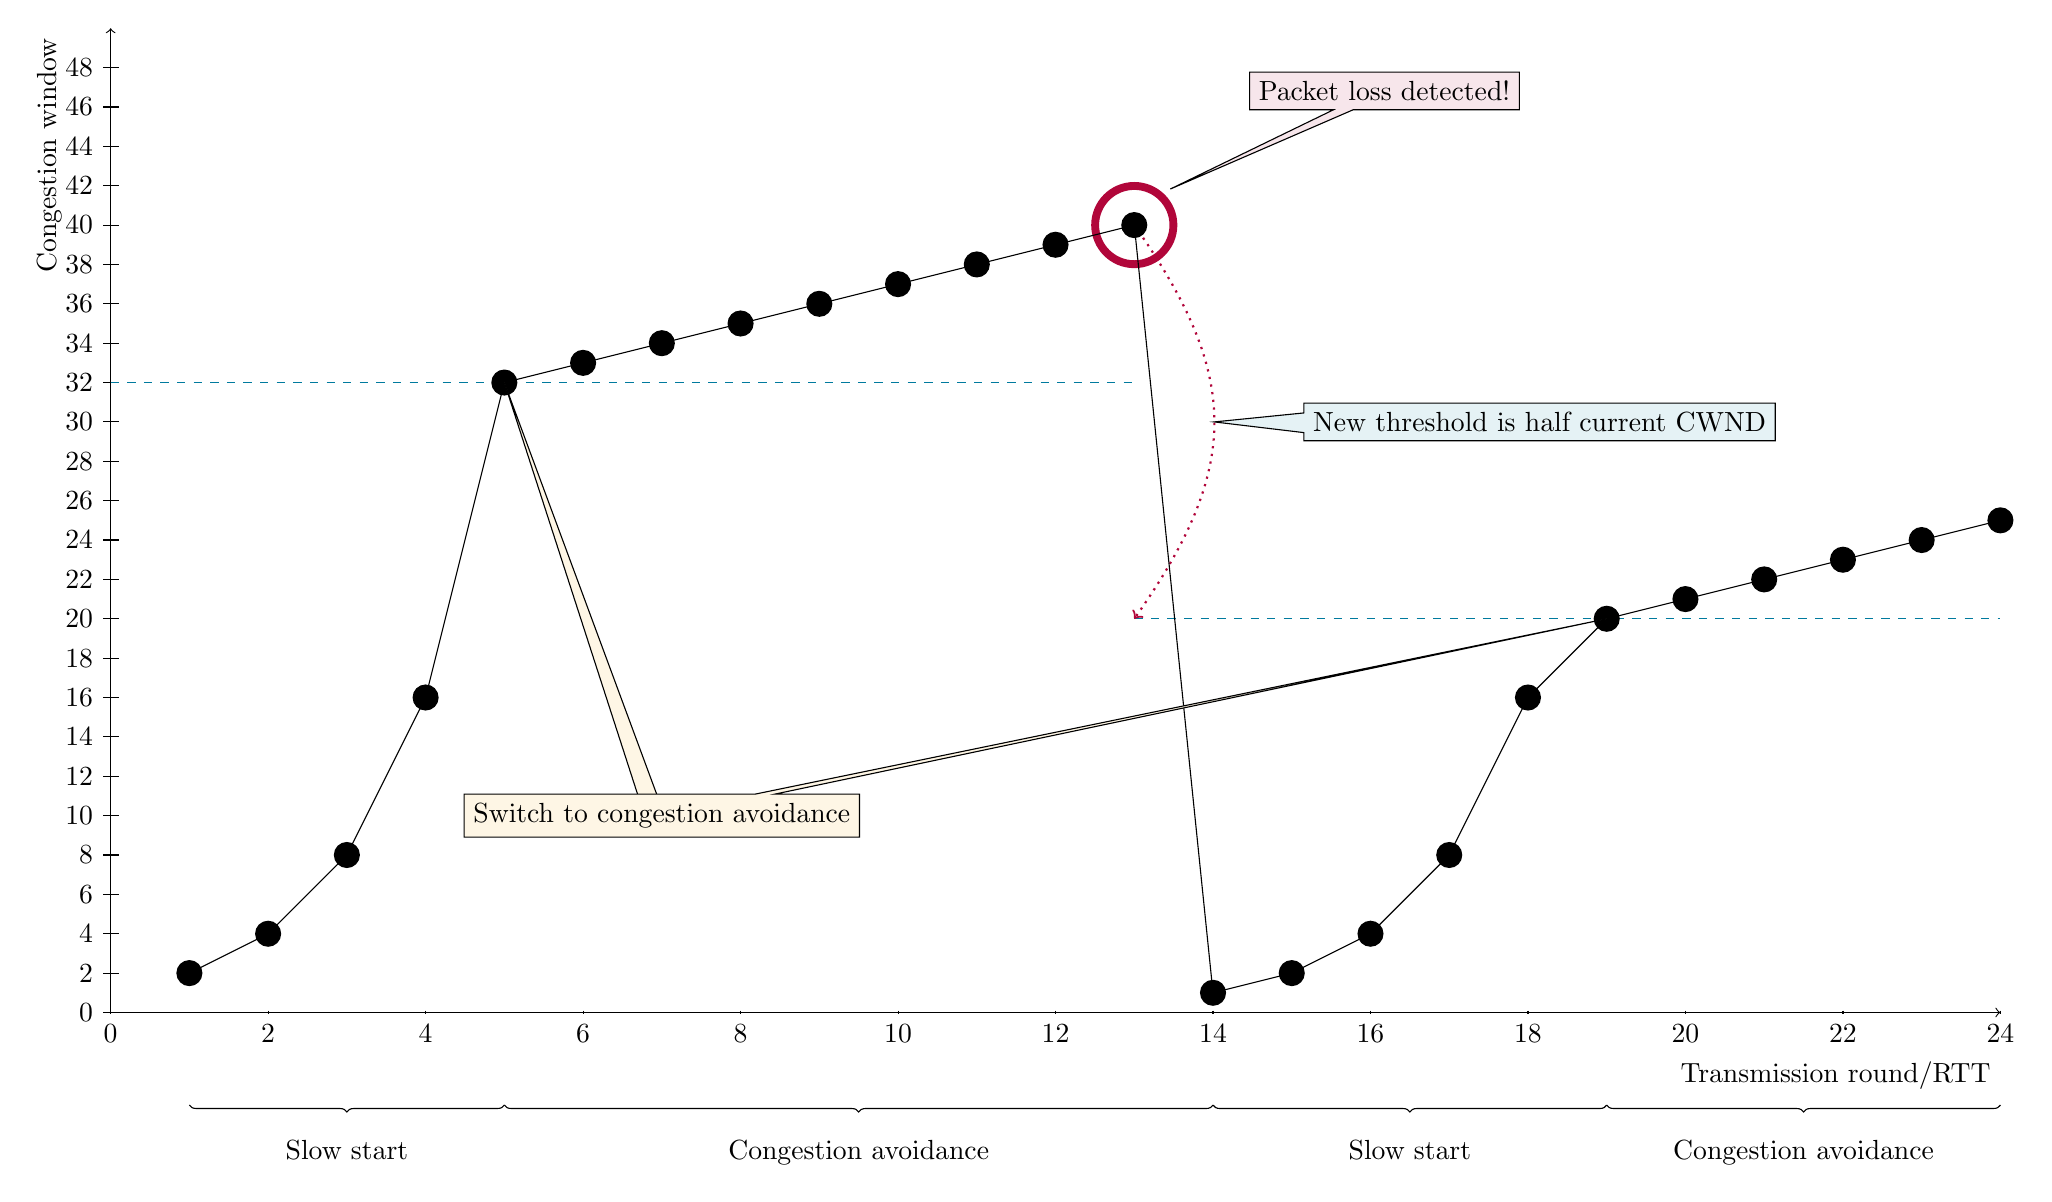
\begin{tikzpicture}[yscale=0.25]
  \label{page:cc:tahoe}
  \draw [->] (0,0)  -- (0, 50) node [left=0.5, rotate=90, anchor=south east] {Congestion window};
  \foreach \i in {0,2,...,48} {
    \draw (0.1,\i) -- (-0.1,\i) node [left] {\i}; 
  }

  \draw [->] (0,0) -- (24,0) node [below=0.5,anchor=north east] {Transmission round/RTT};
  \foreach \i in {0,2,...,24} {
    \draw (\i, 0.1) -- (\i, -0.1) node [below] {\i}; 
  }
 
  % packet loss detected
  \node [draw=hpired, scale=3, line width=1mm, circle]  (pl) at (13, 40) {}; 
  \node [rectangle callout, fill=hpired!10, draw,
  callout absolute pointer={(pl.north east)},
  above right=of pl]  {Packet loss detected!}; 
  
  % sstart threshold 
  \draw [dashed, hpiblue] (0,32) -- (13,32); 
  \draw [dashed, hpiblue] (13,20) -- (24,20); 
  \draw [hpired, dotted, thick, ->] (13, 40) to [bend left=10, ] node (halfss) {} (13, 20);
  \node [rectangle callout, fill=hpiblue!10, draw,
  callout absolute pointer={(halfss)},
  right=of halfss] {New threshold is half current CWND}; 
  
  % sequence of nodes: 
  \node [circle, fill] at (1, 2) (n1) {};
  \foreach \t/\c [remember=\c as \lastc (initially 2), remember=\t as \lastt (initially 1), ] in {2/4, 3/8, 4/16,5/32, 6/33, 7/34, 8/35, 9/36, 10/37, 11/38, 12/39, 13/40, 14/1,15/2,16/4, 17/8, 18/16, 19/20,  20/21, 21/22, 22/23, 23/24, 24/25} {
    \draw (\lastt, \lastc) -- (\t, \c) node [circle, fill] (n\t) {}; 
  }

  \node [rectangle callout, fill=hpiyellow!10, draw,
  callout absolute pointer={(5, 32)}] at (7,10) {}; 
  
  \node [rectangle callout, fill=hpiyellow!10, draw,
  callout absolute pointer={(19, 20)}] at (7,10) {Switch to congestion avoidance};

  % mark the various phases
  \draw [decorate, decoration={brace, raise=5pt, mirror}] (1,-4) to node[below=0.5] {Slow start} (5, -4) ; 
  \draw [decorate, decoration={brace, raise=5pt, mirror}] (5,-4) to node[below=0.5] {Congestion avoidance} (14, -4) ; 
  \draw [decorate, decoration={brace, raise=5pt, mirror}] (14,-4) to node[below=0.5] {Slow start} (19, -4) ; 
  \draw [decorate, decoration={brace, raise=5pt, mirror}] (19,-4) to node[below=0.5] {Congestion avoidance} (24, -4) ; 
  

\end{tikzpicture}


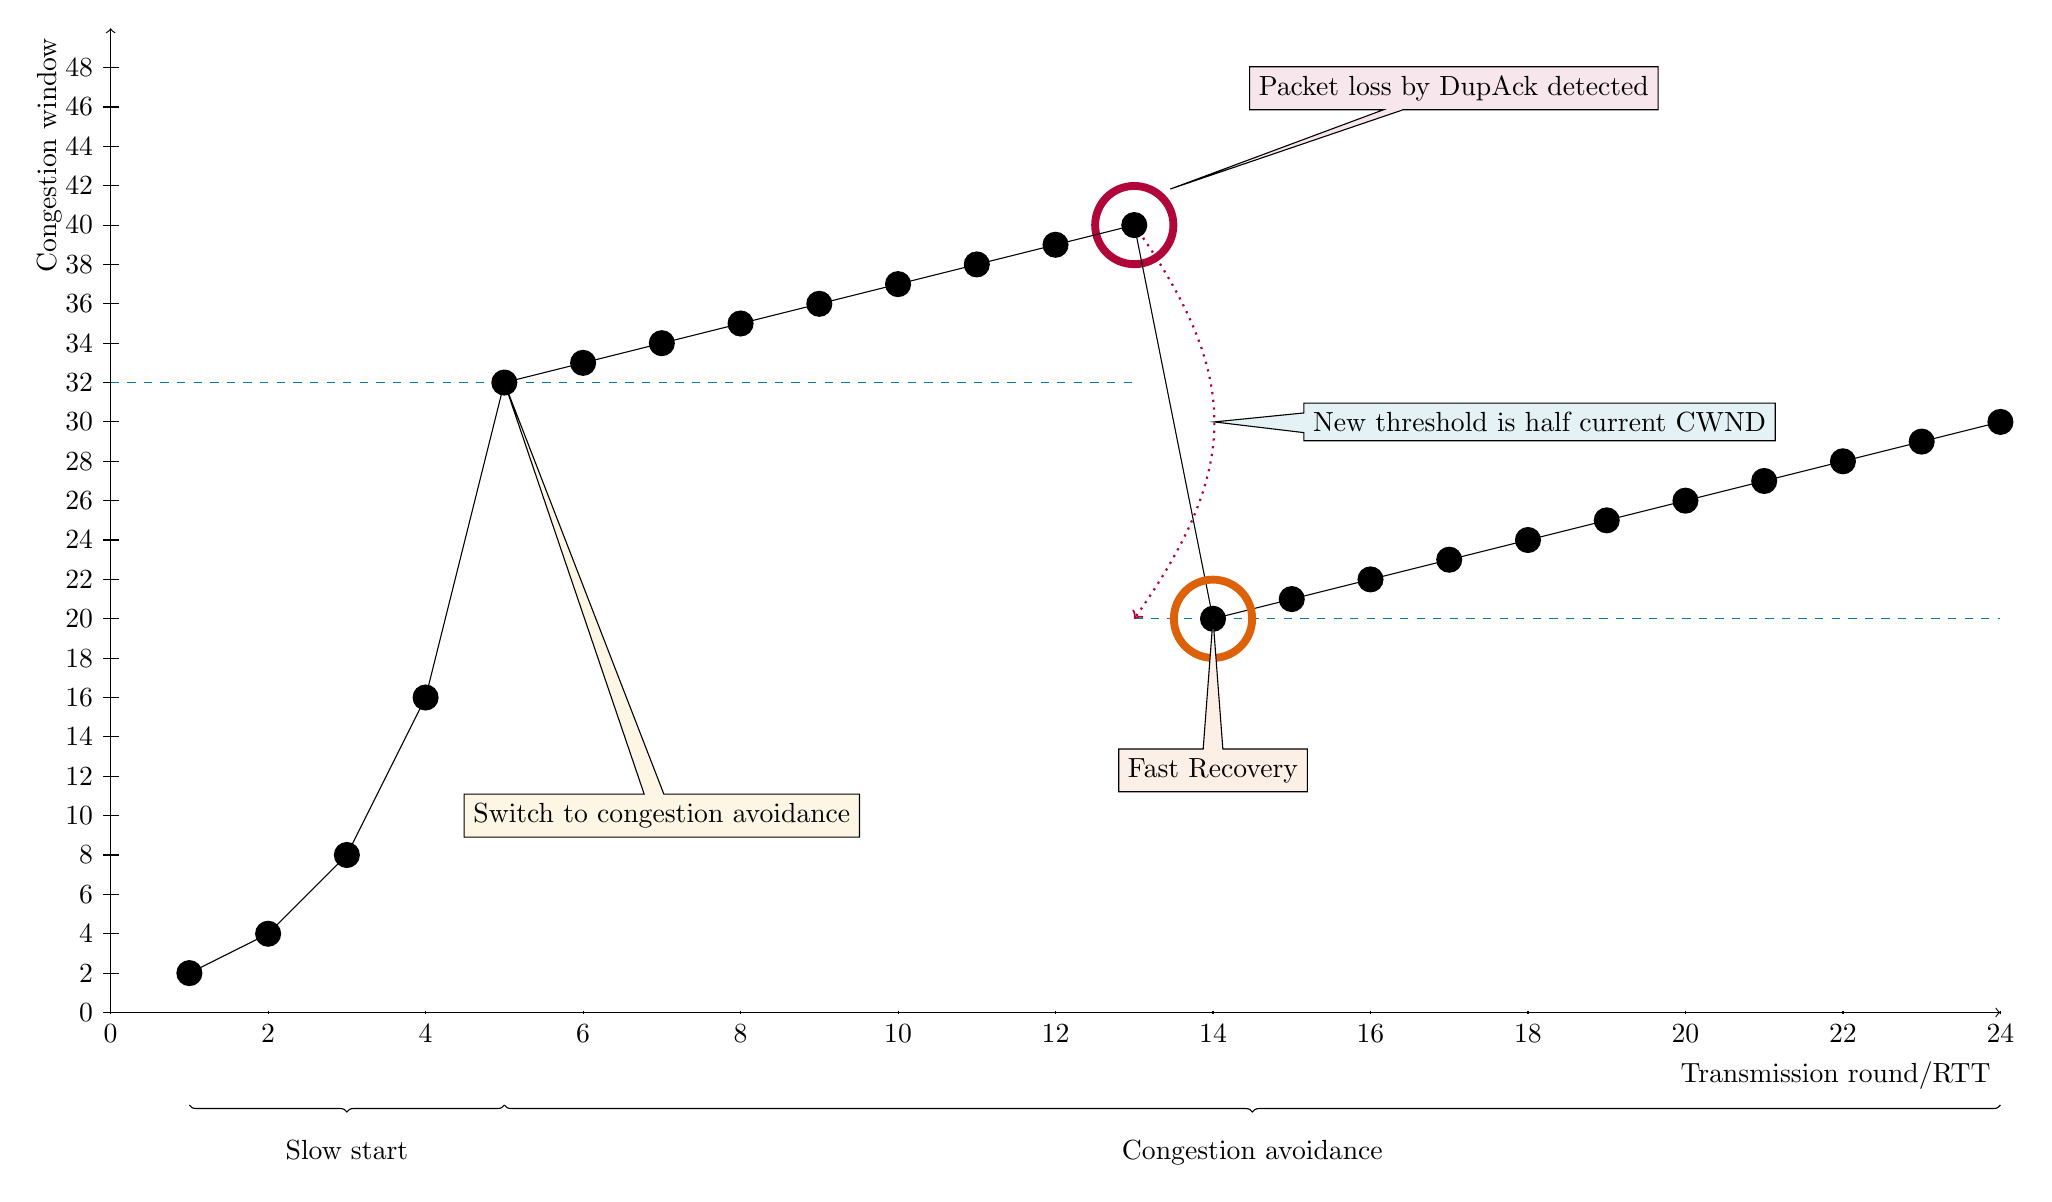
\begin{tikzpicture}[yscale=0.25]
  \label{page:cc:reno}

  \draw [->] (0,0)  -- (0, 50) node [left=0.5, rotate=90, anchor=south east] {Congestion window};
  \foreach \i in {0,2,...,48} {
    \draw (0.1,\i) -- (-0.1,\i) node [left] {\i}; 
  }

  \draw [->] (0,0) -- (24,0) node [below=0.5,anchor=north east] {Transmission round/RTT};
  \foreach \i in {0,2,...,24} {
    \draw (\i, 0.1) -- (\i, -0.1) node [below] {\i}; 
  }
 
  % packet loss detected
  \node [draw=hpired, scale=3, line width=1mm, circle]  (pl) at (13, 40) {}; 
  \node [rectangle callout, fill=hpired!10, draw,
  callout absolute pointer={(pl.north east)},
  above right=of pl]  {Packet loss by DupAck detected}; 
  
  % sstart threshold 
  \draw [dashed, hpiblue] (0,32) -- (13,32); 
  \draw [dashed, hpiblue] (13,20) -- (24,20); 
  \draw [hpired, dotted, thick, ->] (13, 40) to [bend left=10, ] node (halfss) {} (13, 20);
  \node [rectangle callout, fill=hpiblue!10, draw,
  callout absolute pointer={(halfss)},
  right=of halfss] {New threshold is half current CWND}; 
  
  % sequence of nodes: 
  \node [circle, fill] at (1, 2) (n1) {};
  \foreach \t/\c [remember=\c as \lastc (initially 2), remember=\t as \lastt (initially 1), ] in {2/4, 3/8, 4/16,5/32, 6/33, 7/34, 8/35, 9/36, 10/37, 11/38, 12/39, 13/40, 14/20,15/21,16/22, 17/23, 18/24, 19/25,  20/26, 21/27, 22/28, 23/29, 24/30} {
    \draw (\lastt, \lastc) -- (\t, \c) node [circle, fill] (n\t) {}; 
  }

  \node [rectangle callout, fill=hpiyellow!10, draw,
  callout absolute pointer={(5, 32)}] at (7,10) {Switch to congestion avoidance}; 

  \node [hpiorange, circle, scale=3, draw, line width=1mm] at (14,20) (fr) {};
  \node [rectangle callout, fill=hpiorange!10, draw,
  callout absolute pointer={(fr)}, below=of fr]  {Fast Recovery}; 
  

  % mark the various phases
  \draw [decorate, decoration={brace, raise=5pt, mirror}] (1,-4) to node[below=0.5] {Slow start} (5, -4) ; 
  \draw [decorate, decoration={brace, raise=5pt, mirror}] (5,-4) to node[below=0.5] {Congestion avoidance} (24, -4) ; 
  

\end{tikzpicture}


\end{document}